\documentclass{beamer}
\usepackage{beamerthemesplit}
\usepackage{wrapfig}
\usetheme{SPbGU}
\usepackage{pdfpages}
\usepackage{amsmath}
\usepackage{cmap} 
\usepackage[T2A]{fontenc} 
\usepackage[utf8]{inputenc}
\usepackage[english,russian]{babel}
\usepackage{indentfirst}
\usepackage{amsmath}
\usepackage{tikz}
\usepackage{multirow}
\usepackage{algorithm}
\usepackage{algorithmicx}
\usetikzlibrary{shapes,arrows}
\usepackage{fancyvrb}
\usepackage{graphicx}
\usepackage{graphics}

\newtheorem{rutheorem}{Теорема}
\newtheorem{ruproof}{Доказательство}
\newtheorem{rudefinition}{Определение}
\newtheorem{rulemma}{Лемма}
\beamertemplatenavigationsymbolsempty

\title[]{Реализация и оценка эффективности алгоритма
	обобщенного синтаксического анализа с уменьшенной
	активностью стека}
\subtitle[]{}
% То, что в квадратных скобках, отображается в левом нижнем углу. 
\institute[СПбГУ]{
Санкт-Петербургский государственный университет \\
Кафедра системного программирования }

% То, что в квадратных скобках, отображается в левом нижнем углу.
\author[Дмитрий Ковалев]{Дмитрий Ковалев, 344 группа \\
  % У научного руководителя должна быть указана научная степень
  \and  
    {\bfseries Научный руководитель:} магистр информационных технологий, ст.пр. Григорьев С.В. \\ 
  % Для курсовой не обязателен. Должна быть указана должность или ученая степень
}

\date{08 сентября 2016г.}

\definecolor{orange}{RGB}{179,36,31}

\begin{document}
\setbeamertemplate{caption}{\raggedright\insertcaption\par}
{
% Лого университета или организации, отображается в шапке титульного листа
\begin{frame}
  \begin{center}
  {
\includegraphics[width=1.5cm]{pictures/SPbGU_Logo.png}}
  \end{center}
  \titlepage
\end{frame}
}

\begin{frame}[fragile]
  \transwipe[direction=90]
  \frametitle{Неоднозначные КС-грамматики}
  \begin{itemize}
    \item Области применения
	\begin{itemize}
		\item Синтаксический анализ динамически формируемого кода
		\item Биоинформатика
	\end{itemize}
	\item Алгоритмы
	\begin{itemize}
		\item CYK
		\item Earley
		\item Generalized LR (GLR)
		\item RNGLR
	\end{itemize}
    \item Недостаток --- скорость
  \end{itemize}
\end{frame}
            
\begin{frame}
  \transwipe[direction=90]
  \frametitle{Reduction Incorporated GLR (RIGLR)}
  \begin{itemize}
    \item Сводит использование стека к обработке вложенной рекурсии
    $$ A \Rightarrow ... \Rightarrow \alpha A \beta, \ \alpha, \beta \neq \epsilon $$
    \item Позволяет с меньшими затратами анализировать регулярную
    часть языка
    \item Scott, E. and Johnstone, A.``Generalized Bottom Up Parsers With Reduced Stack Activity'', Computer Journal
  \end{itemize}
\end{frame}

\begin{frame}
	\transwipe[direction=90]
	\frametitle{YaccConstructor (YC)}
	\begin{itemize}
		\item Проект лаборатории языковых инструментов  JetBrains, направленный на исследования в области формальных языков, лексического и синтаксического анализов
		\item .NET, F$\#$
		\item Синтаксический анализ динамически формируемого кода на основе RNGLR
	\end{itemize}
\end{frame}

% Обязательный слайд: четкая формулировка цели данной работы и постановка задачи
% Описание выносимых на защиту результатов, процесса или особенностей их достижения и т.д.
\begin{frame}
  \transwipe[direction=90]
  \frametitle{Постановка задачи}
  \textbf{Целью} данной работы является увеличение производительности алгоритма синтаксического анализа динамически формируемого кода
  \textbf{Задачи}:
  \begin{itemize}
    \item Изучить RIGLR-алгоритм синтаксического анализа
    \item Реализовать генератор синтаксических анализаторов, основанный на RIGLR-алгоритме
    \item Провести сравнение производительности анализаторов, созданных на основе RNGLR и RIGLR    
  \end{itemize}
\end{frame}

\begin{frame}[fragile]
	\transwipe[direction=90]
	\frametitle{Архитектура платформы}
	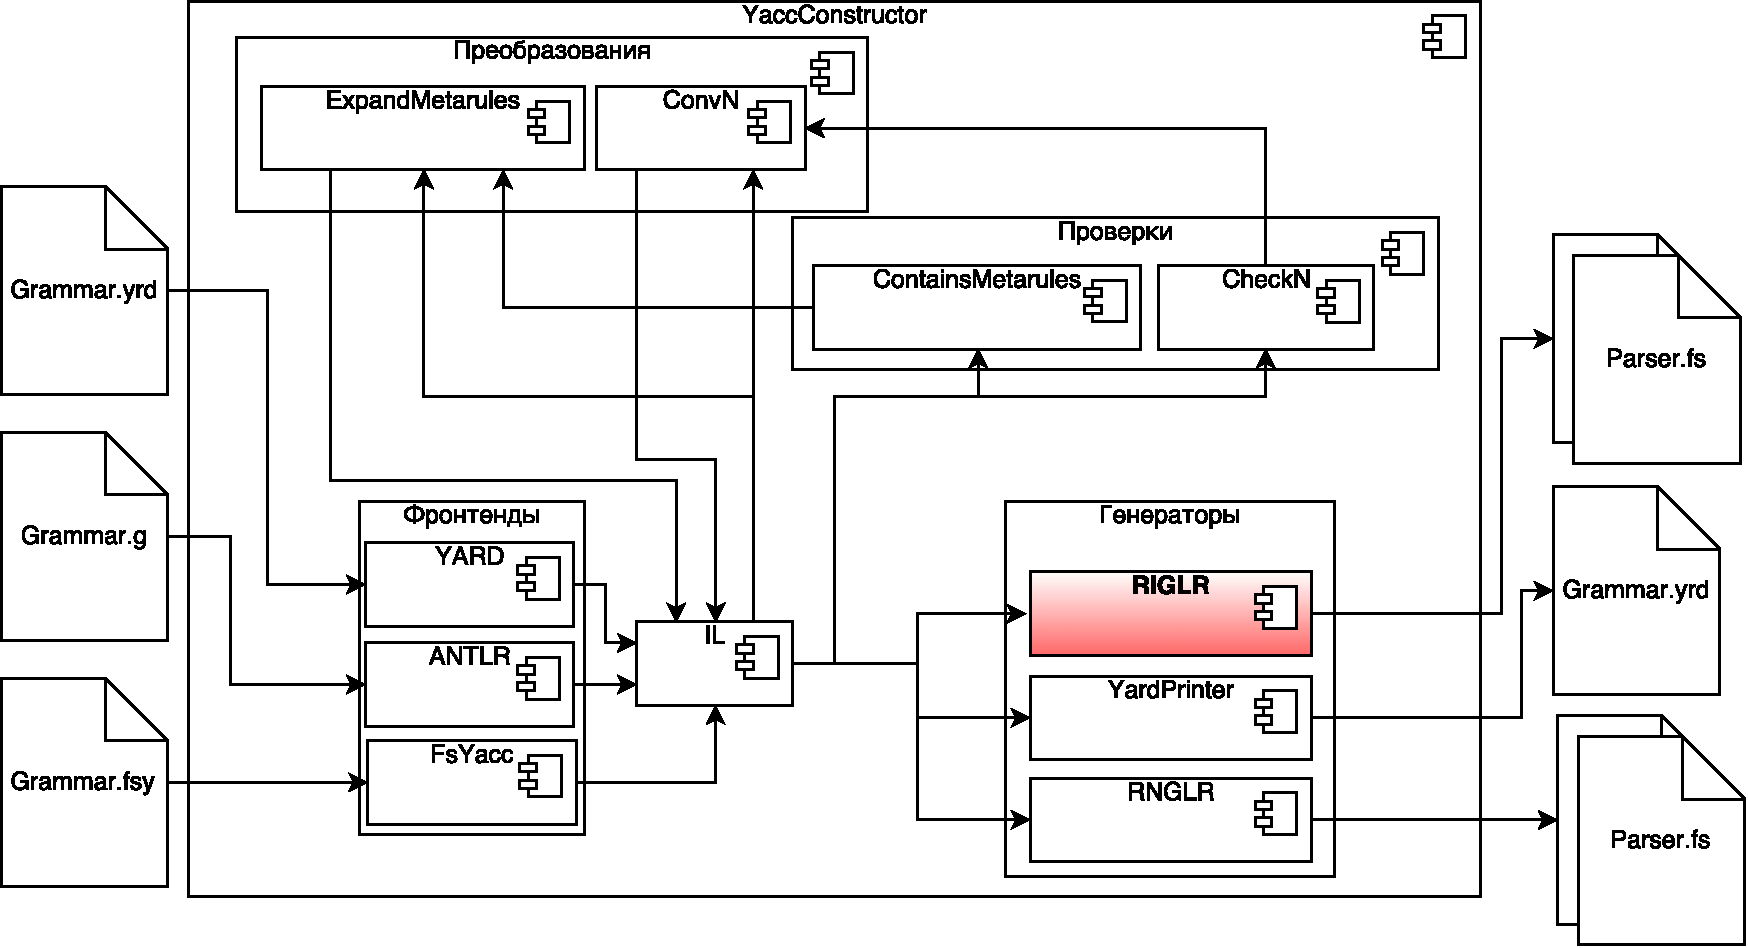
\includegraphics[width=12cm]{pictures/YCArch.pdf}
\end{frame}

\begin{frame}[fragile]
	\transwipe[direction=90]
	\frametitle{Архитектура RIGLR-модуля}
	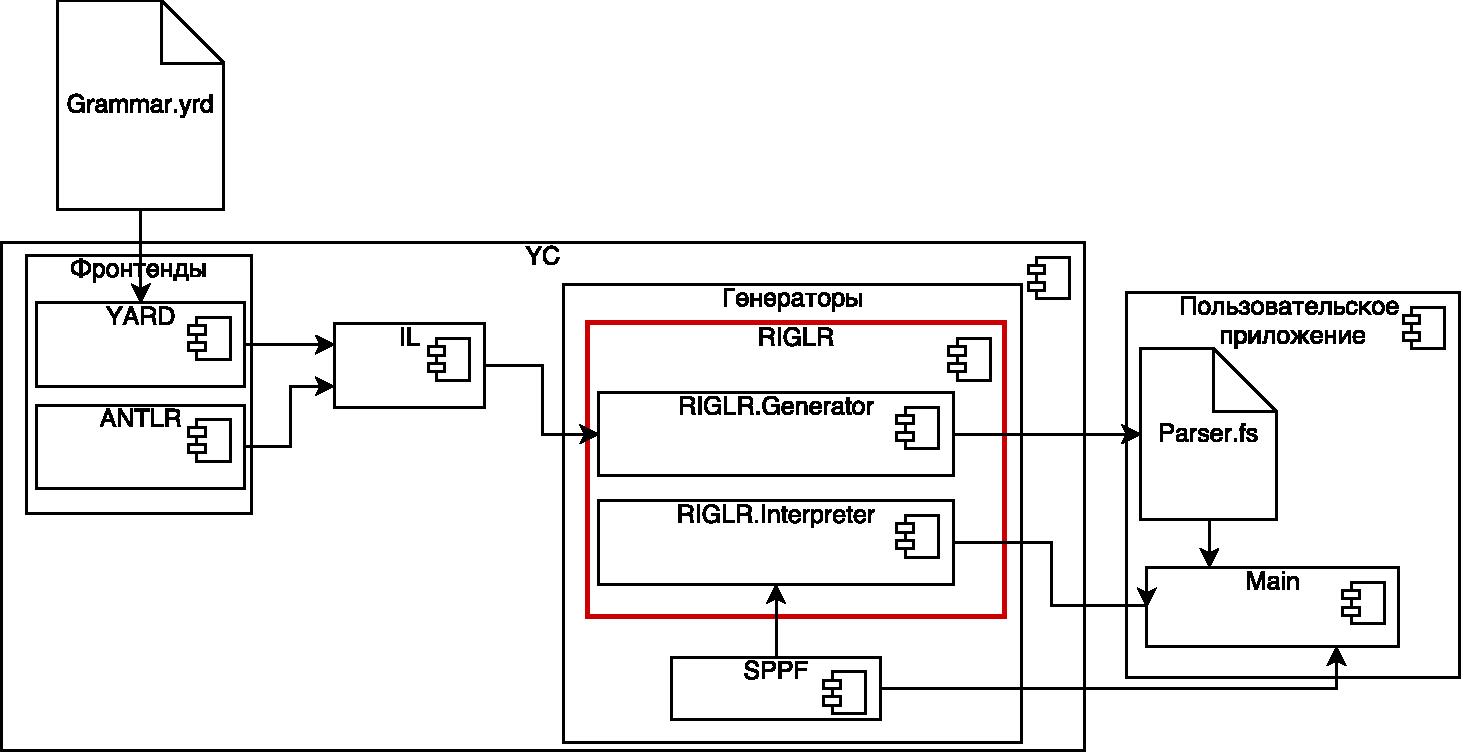
\includegraphics[width=12cm]{pictures/RIGLRArch.pdf}
\end{frame}

\begin{frame}
	\transwipe[direction=90]
	\frametitle{Подробности реализации}
	\begin{itemize}
		\item Модуль генератора
		\begin{itemize}
			\item Реализация автоматов, необходимых для создания управляющих таблиц (QuickGraph)
			\item Алгоритм удаления вложенной рекурсии \footnote{Marcella Anselmo, Dora Giammarresi, and Stefano Varricchio. 2002. Finite automata and non-self-embedding grammars.}
			\item Генерация файла, содержащего таблицы и дополнительную информацию для парсера
		\end{itemize}
		\item Модуль интерпретатора
		\begin{itemize}
			\item Основная логика RIGLR-анализатора
		\end{itemize}
	\end{itemize}	
\end{frame}

\begin{frame}[fragile]
	\transwipe[direction=90]
	\frametitle{Эксперименты}
	\begin{itemize}
		\item Сильно неоднозначная грамматика, инициирует худший случай работы
		$$ 
		\begin{array}{crcl}
			&start &::=& s \\
			&s & ::= & s \ s \ s \ | \ s \ s \ | \ A\\
		\end{array} 
		$$	
		\item Характеристики компьютера
		\begin{itemize}
			\item Процессор: Intel(R) Core(TM) i7-4790 CPU 3.60GHz, 4 Core(s)
			\item Оперативная память: 16.0 GB DDR3
		\end{itemize}
	\end{itemize}
\end{frame}

\begin{frame}[fragile]
	\transwipe[direction=90]
	\frametitle{Эксперименты}
	\begin{figure}[!tbp]
		\centering
		\begin{minipage}[h]{0.3\textwidth}
			\begin{table}[b]
				\centering
				\resizebox{\columnwidth}{!}{
				\begin{tabular}{|l|l|l|}
					\hline				
					Токены & RNGLR & RIGLR  \\ \hline
					10     & 30    & 20     \\ \hline
					20     & 60    & 40     \\ \hline
					30     & 90    & 60     \\ \hline
					40     & 120   & 80     \\ \hline
					50     & 150   & 100    \\ \hline
				\end{tabular}
				}								
				\caption{Кол-во вершин в стеке}
				\label{stack_table}
			\end{table} 			
		\end{minipage}
		\hfill
		\begin{minipage}[h]{0.65\textwidth}
			\begin{figure}[c]
				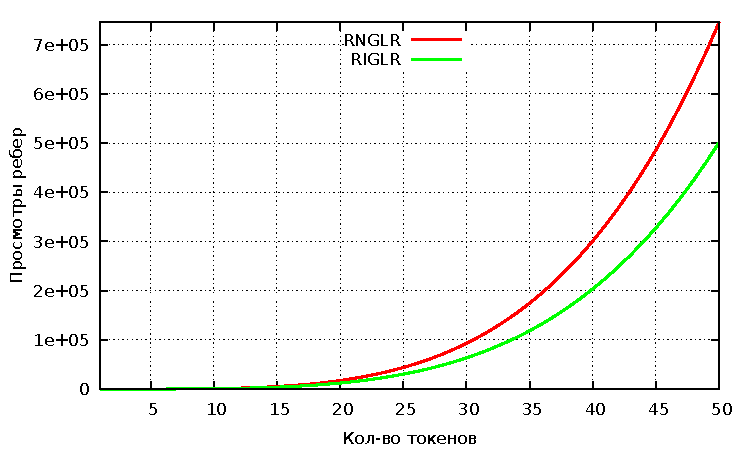
\includegraphics[width=\textwidth]{pictures/edge_visit.pdf}
				\caption{Количество просмотров ребер стека}
			\end{figure}			
		\end{minipage}
	\end{figure}
\end{frame}

\begin{frame}[fragile]
	\transwipe[direction=90]
	\frametitle{Эксперименты}
	\begin{figure}
		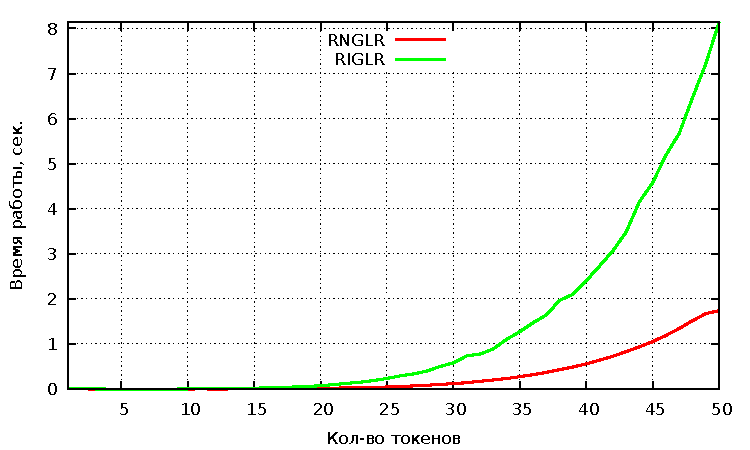
\includegraphics[width=0.9\textwidth]{pictures/time.pdf}
		\caption{Время работы}
	\end{figure}
\end{frame}

\begin{frame}
  \transwipe[direction=90]
  \frametitle{Результаты}
  В ходе данной работы получены следующие результаты
  \begin{itemize}
    \item Изучен RIGLR-алгоритм синтаксического анализа
    \item Реализован генератор синтаксических анализаторов, основанный на RIGLR-алгоритме
    \item Проведено сравнение производительности анализаторов, созданных на основе RNGLR и RIGLR  
  \end{itemize}
  Исходный код работы может быть найден в репозитории YC на GitHub (\hyperlink{a}{https://github.com/YaccConstructor/YaccConstructor}). Автор работал под учетной записью $Lares77$.
\end{frame}

\end{document}
